\documentclass[12pt]{article}
 
\newenvironment{sol}[1][Solution]{\begin{trivlist}\item[\hskip\labelsep {\bfseries #1:}]}{\end{trivlist}}
\usepackage{minted}
%\usemintedstyle{perldoc}
\usemintedstyle{vs}
\usepackage{graphicx}
\graphicspath{./}

\usepackage[margin=1in]{geometry} 
\usepackage{amsmath,amsthm,amssymb}
\usepackage{times,url}
\usepackage{tikz}
\usepackage{enumerate}
\begin{document}
\renewcommand{\qedsymbol}{\filledbox}
\begin{center}
    \textbf{CS 5/7350 - Test\#1} \\
    \textbf{March, 2020}
%replace X with the appropriate number
\end{center}
\begin{flushright}
Name: \underline{Bingying Liang }\\
ID:  \underline{\ \ \ \ \ 48999397 \ \ \ \ \ }
\end{flushright}
\begin{enumerate}
    \item \ [9 pts] Define the following Terms as succinctly as possible:
    \begin{enumerate}
        \item Algorithm:
        \begin{sol}
            A step by step procedure for solving a problem in \textbf{a finite amount of time}.
        \end{sol}

        \item Tree
        \begin{sol}
            A connected acyclic graph. (Does not have to be rooted)
        \end{sol}

        \item In-Order Traversal
        \begin{sol}
        Visiting the vertices of a rooted tree by recursively visiting the left subtree, the current vertex and then the right subtree.
        \end{sol}

        \item Graph
        \begin{sol}
        A collection of elements (Vertices) and a relation on those elements(edges)
        \end{sol}

        \item NP-Hard 
        \begin{sol}
        A class of problems that at least as hard (may or may not also be NP problem itself) and some are possibly harder than all NP problems. (solve 1, solve all NP problems).
        \end{sol}

        \item Insertion Sort
        \begin{sol}
            A method of ordering items by taking each item and placing it wher it belongs among the other items already taken.
        \end{sol}
    \end{enumerate}

    \item \ [8 pts] Solve the following problems:
    \begin{enumerate}
        \item $2^{55}$ modulo 11 = 
        \begin{sol}
        10\\
        $2^{55} = (2^{10} \times 2^{10} \times 2^{10} \times 2^{10} \times 2^{10} \times 2^{5}) \bmod 11=(1\times 1\times 1\times 1\times 1 \times 10)=10$ 
        \end{sol}

        \item \textcolor{red}{Given $|M|= 6 \& |N| = 5$, find $| \text{Power Set of} (M\times N) |$} 
        \begin{sol}
        \begin{align*}
            2^n = 2^{M\times N} = 2^{30}
        \end{align*}
        \end{sol}

        \item Number of edges in a complete graph with 10 vertices = 
        \begin{sol}
            45
        \end{sol}

        \item \ \textcolor{red}{ – ( 1/4 ) modulo 7 = }
        \begin{sol}
            5 \\
            \begin{align*}
                (-\frac{1}{4} \times 4) \bmod 7 = (-1) \bmod 7 = 6\\
                (4 \times 5) \bmod 7 = 6\\
                \therefore (-\frac{1}{4}) \bmod 7 = 5
            \end{align*}
        \end{sol}
    \end{enumerate}

    \item \ [14 pts] For each pair below, circle the choice that has the higher asymptotic upper bound. If they are the same, circle “same”.
    \begin{sol}
                 \begin{center}
            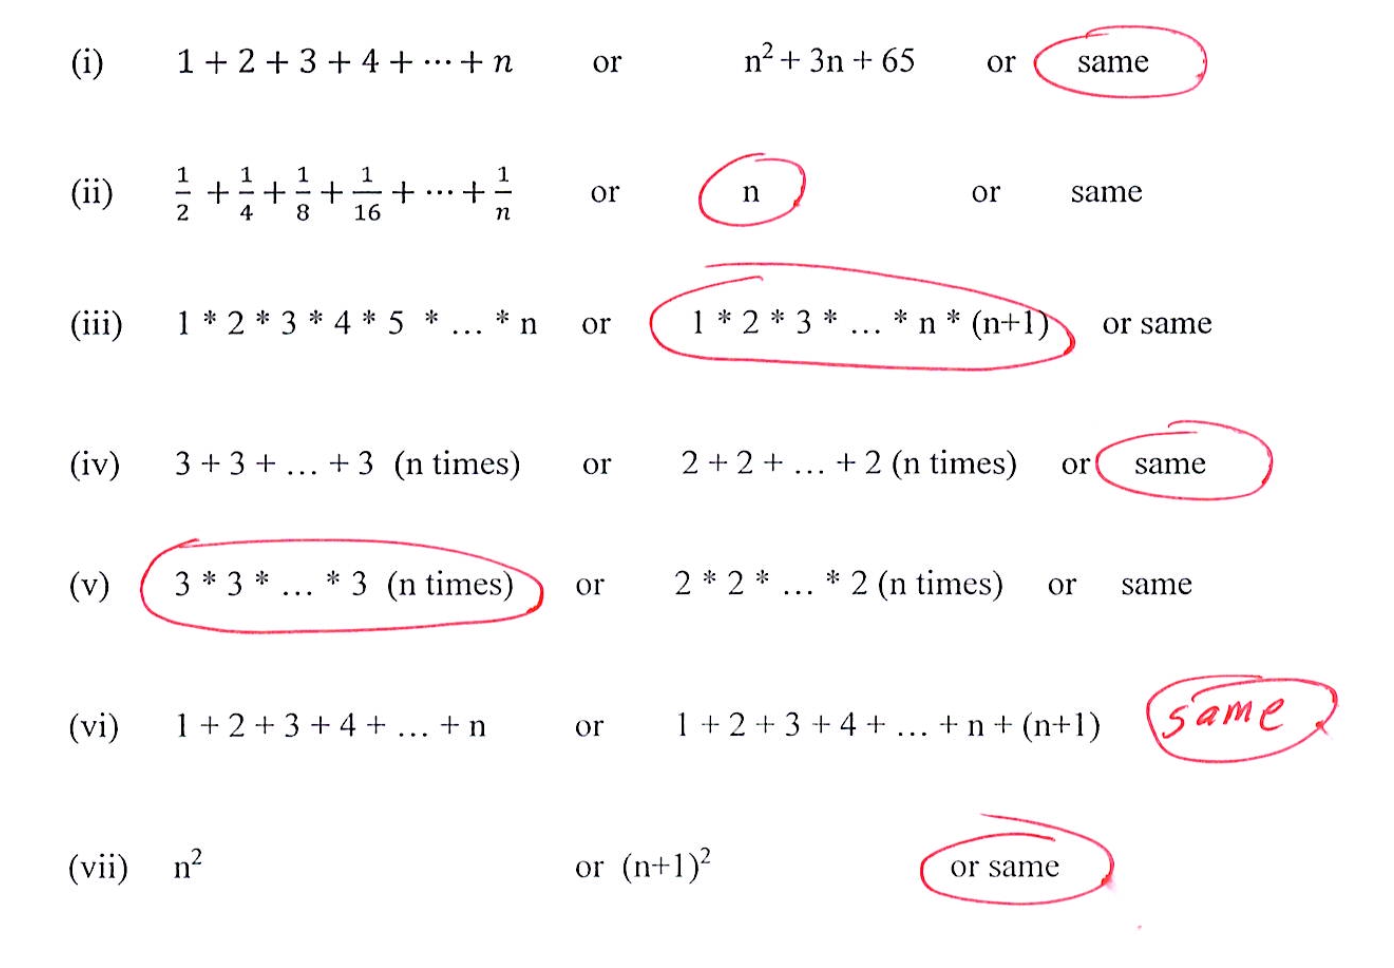
\includegraphics[width = 0.9\textwidth]{p1.png}
    \end{center}
    \end{sol}

    \item \ \textcolor{red}{[5 pts] Argue that the problem, H, of creating a MIN-HEAP from an unsorted array of integers using the HEAPIFY algorithm discussed in class is at least as hard - and maybe even harder - than the problem, M, of finding the minimum element of the same unsorted array of integers.}
    \begin{sol}
        Given a solution to Problem H, I can use that solution to solve problem M by simply reading the first element of the heap created by the solution to H.
    \end{sol}

    \item \ \textcolor{red}{ [9 pts] Determine a Huffman encoding for each symbol in a message that contains:}
    \begin{center}
        8 C's, 8D's, 3 E's, 3 F's, 2G's, 1H and 1K.
    \end{center}
    \begin{enumerate}
        \item How many bits are in the entire message if each symbol is encoded with 3 bits? 
        \begin{sol}
        \begin{align*}
            (8 + 8 + 3 + 3 + 2 + 1+ 1) \times 3 = 26 \times 3 = 78 \ bits
        \end{align*}
        \end{sol}
        \item How many bits are in the entire Huffman coded message?

        \item How much entropy (information) is in the entire message?
                \begin{sol}
        \hspace*{\fill}\\
                             \begin{center}
            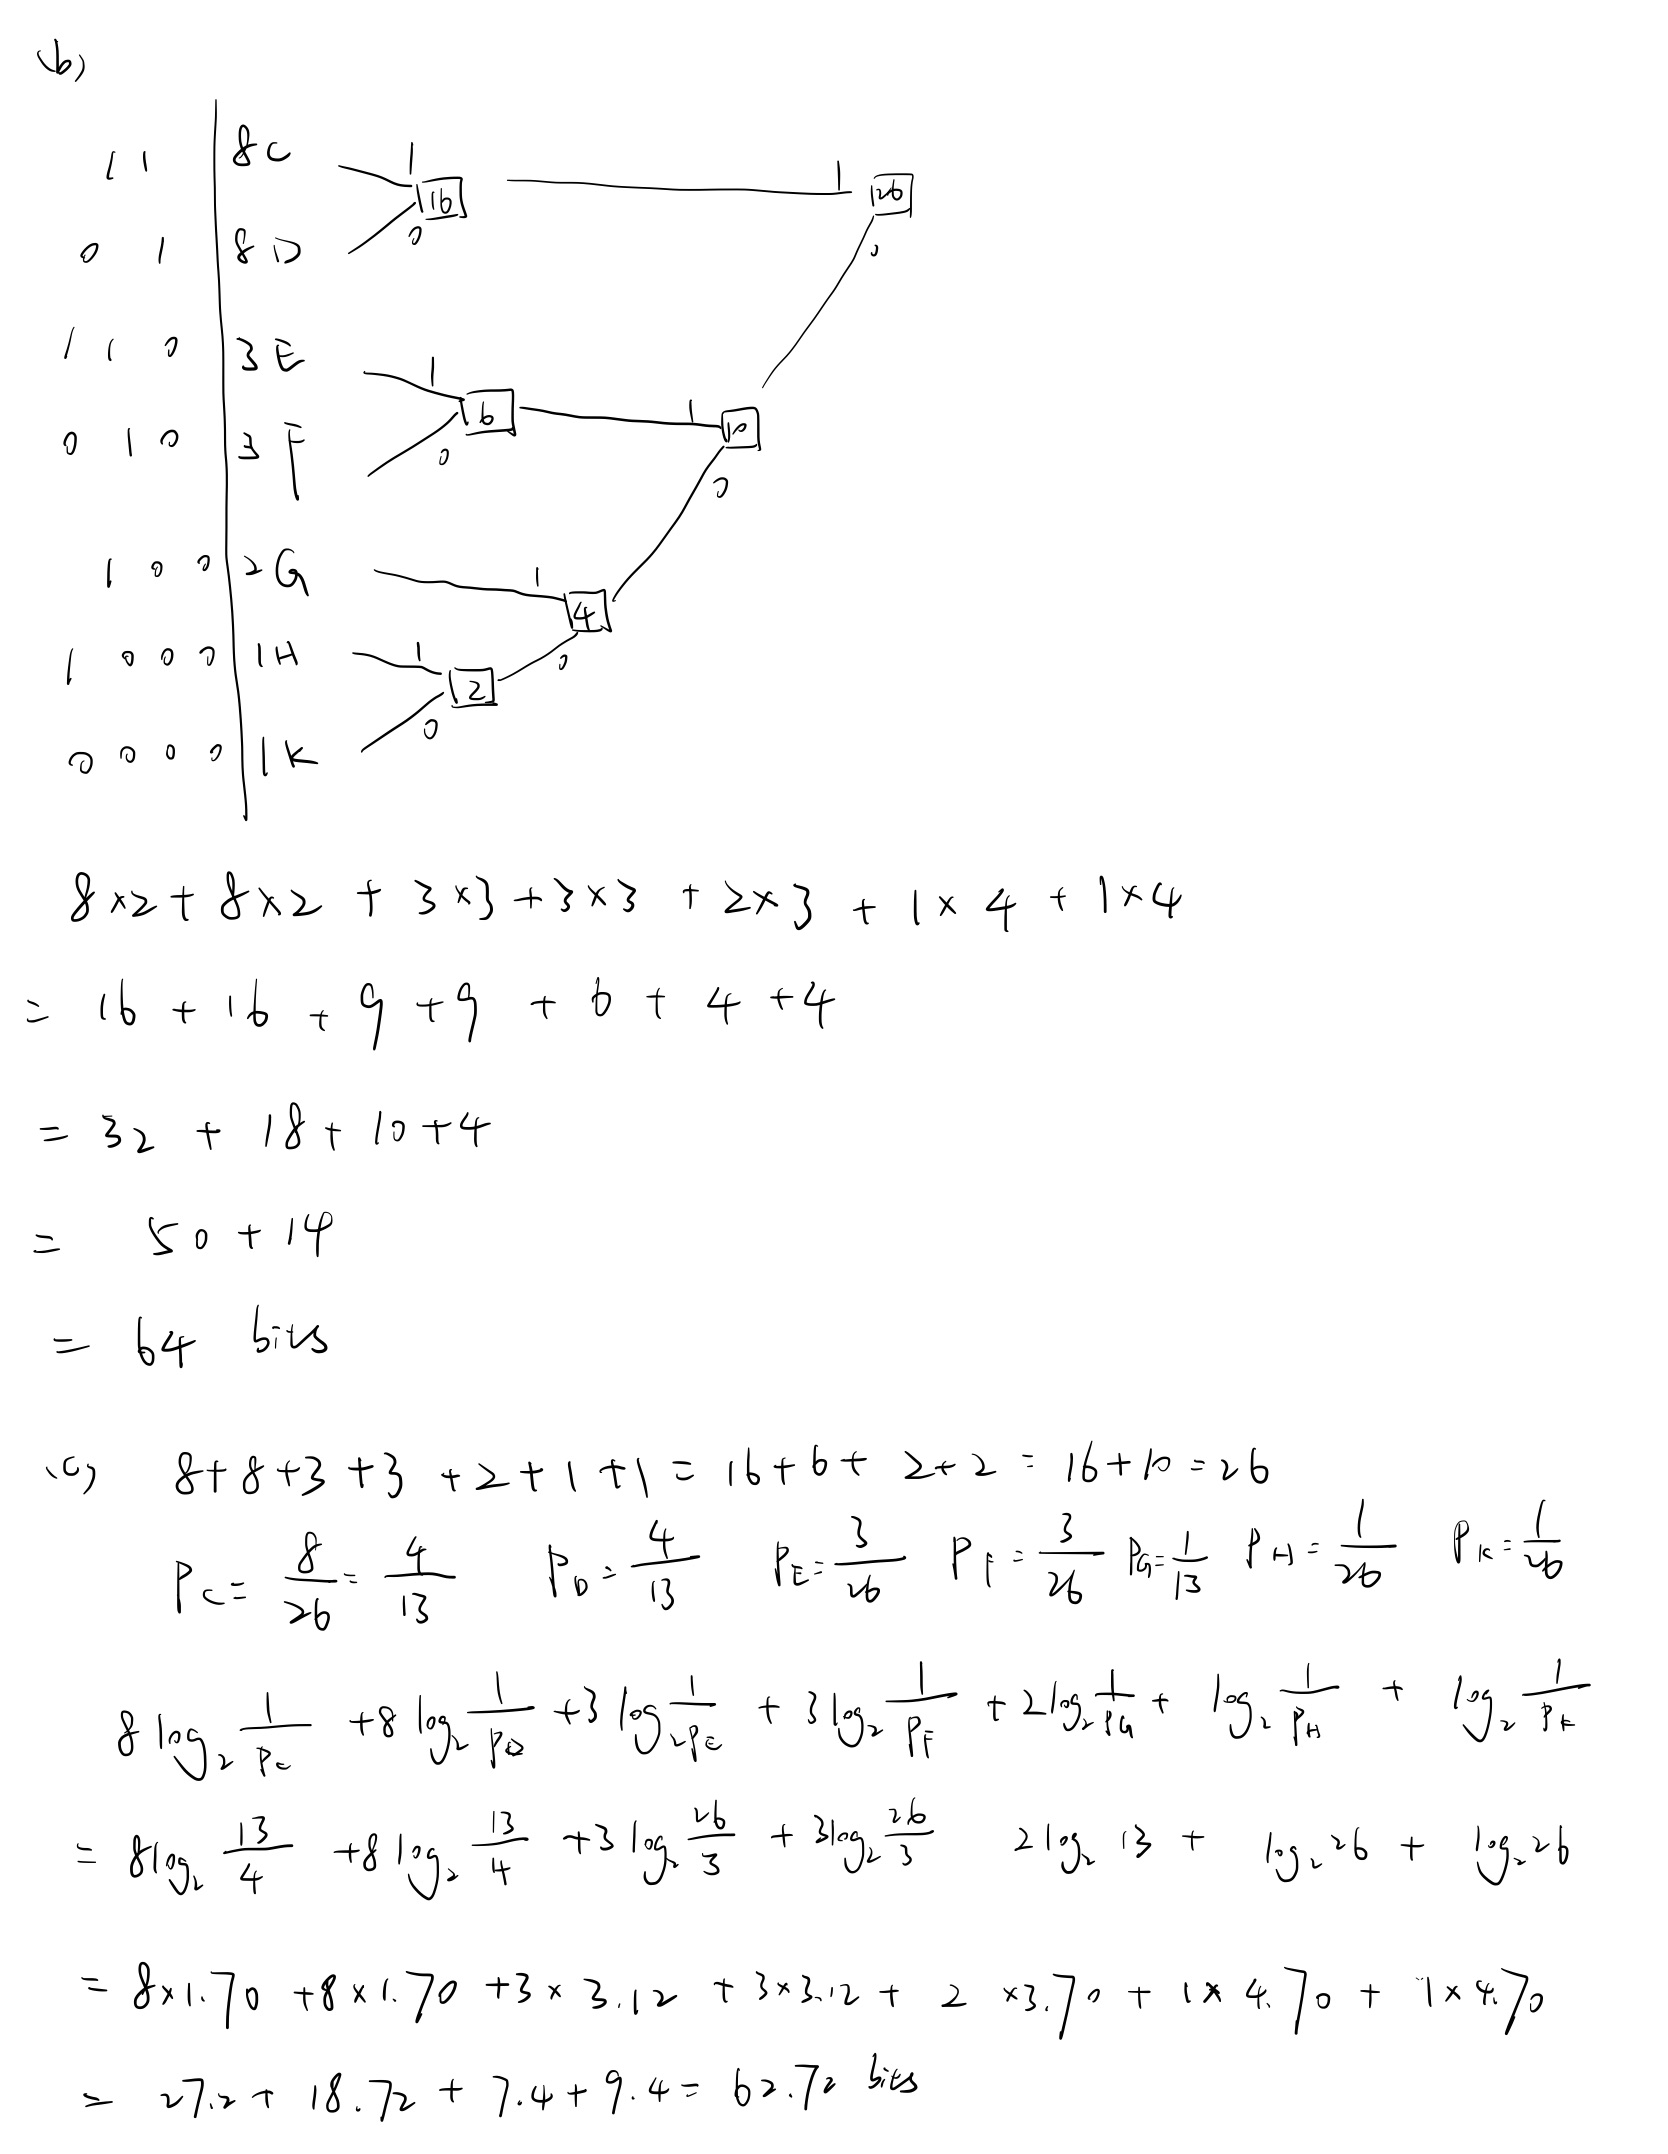
\includegraphics[width = 0.9\textwidth]{p2.jpg}
    \end{center}
        \end{sol}
    \end{enumerate}

    \item \ [6 pts] Two people need to establish a secret key for encrypting communications. They agree to use a Diffie-Hellman key exchange with a modulus of 11 and decide on 2 as the base. Person A chooses a random value of 8 and person B chooses a random value of 9.
    \begin{enumerate}
        \item What is the value Person A sends to Person B
        \begin{sol}
        3
        \end{sol}
        \item What is the value Person B sends to Person A
                \begin{sol}
        6
        \end{sol}
        \item What is the shared secret key between Person A and Person B
                \begin{sol}
        4
        \end{sol}


    \end{enumerate}
    \item \ \textcolor{red}{[ 9 pts] The table below gives asymptotic bounds on various cases of 3 algorithms. Add to the table any bounds you can also determine from the bounds given.}
    \begin{center}
            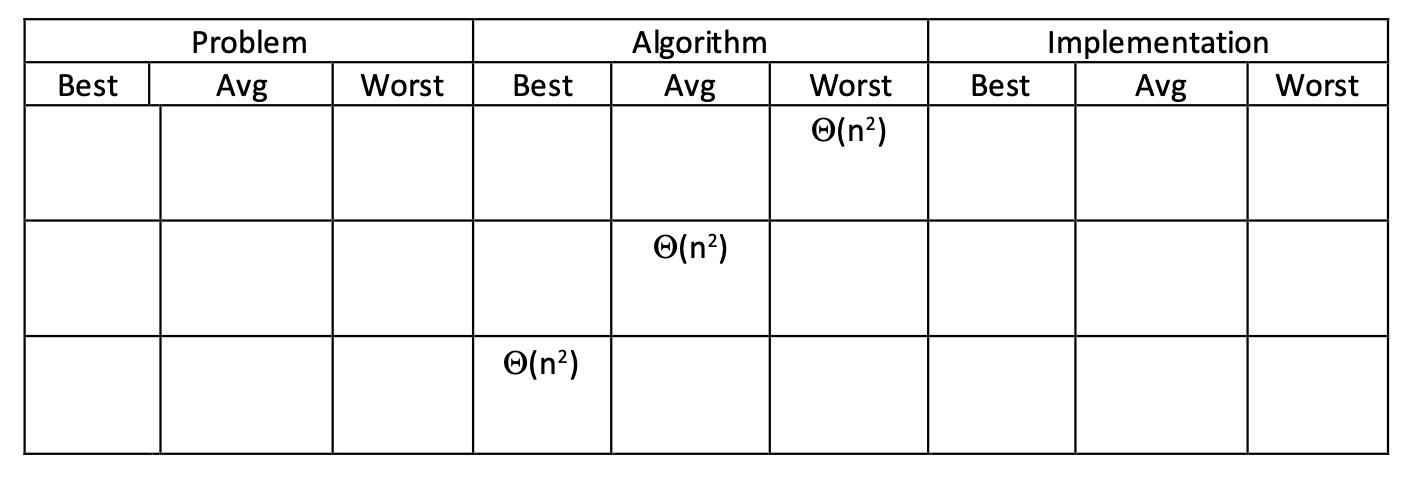
\includegraphics[width = 0.9\textwidth]{p4.png}
    \end{center}
    \begin{sol}
            \begin{center}
            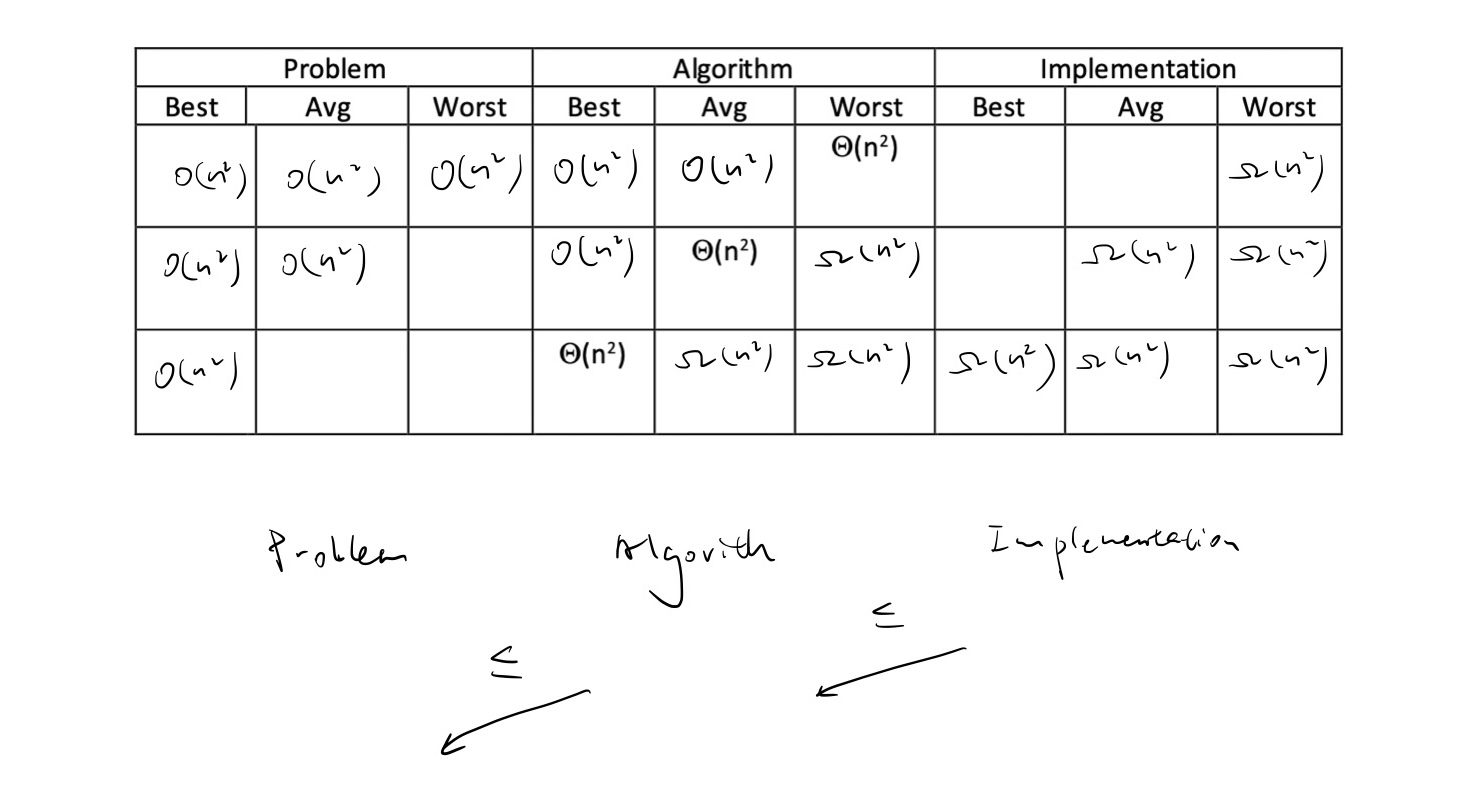
\includegraphics[width = 0.9\textwidth]{p5.jpg}
    \end{center}
    \end{sol}

    \item \ [6 pts] Answer the following questions.:
    \begin{enumerate}
        \item A program requires 6 seconds to process an input size of 45. If the running time is $\Theta(\sqrt{n})$ about how large of an input set could you process in 60s?
        \begin{sol}
            4500 seconds
        \end{sol}

        \item A program requires 5 days to brute force attack a password of 48 bits. Since the running time is $\Theta(2^n)$ about how long would it take for the program to brute force attack a password of 256 bits?
        \begin{sol}
            $5\times 2^{208} $ \textcolor{red}{days}
        \end{sol}

        \item If a program required 5 days to brute force attack a password 48 bits, how long would it take to attack a password of 256 bits if the running time were $O(n^2)$ instead of exponential?
        \begin{sol}
            $142 $ \textcolor{red}{days}
        \end{sol}

    \end{enumerate}

    \item \ \textcolor{red}{[9 pts] Give the tightest asymptotic average case upper and lower bounds you know for the following scenarios:}
    \begin{enumerate}
        \item Deleting the 20th element of an array of size $n$ when order doesn’t matter
        \begin{sol}
            $\Theta(1)$
        \end{sol}

        \item \textcolor{red}{Deleting the 20th element of an array of size $n$ keeping everything else in the same order?}
        \begin{sol}
        $\Theta(n)$\\
        The last one might be the 20th.
        \end{sol}

        \item \textcolor{red}{Finding the k smallest items in an unsorted array of size n}
        \begin{sol}
            $\Theta(n)$ \\
            quick select, just for one time recurtion.
        \end{sol}

        \item \textcolor{red}{Deleting an element from a heap of size n.}
        \begin{sol}
        $\Theta(\log n)$ where n is no of elements in the heap.
        \end{sol}

        \item \textcolor{red}{The best algorithm finding the middle element (based on value) in a sorted array.}
        \begin{sol}
            $\Theta(1)$\\
            Just look it up middle index.
        \end{sol}

        \item The best algorithm searching in a sorted linked list to determine if a specific element (based on value) is present.
        \begin{sol}
                \begin{sol}
        $\Theta(n)$\\
        search all.
        \end{sol}
        \end{sol}
    \end{enumerate}
    
    \item \ [10 pts] Consider the following graph. For any questions needing a starting vertex, use vertex S as the starting vertex.
    \begin{center}
            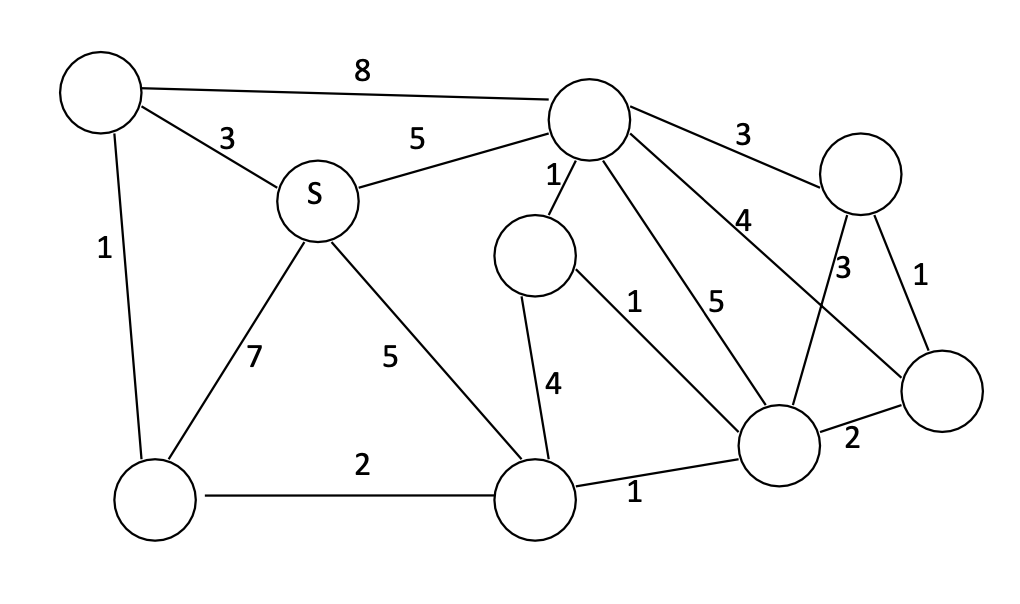
\includegraphics[width = 0.9\textwidth]{p6.png}
    \end{center}
    \begin{enumerate}
        \item What is the value of the third edge chosen when finding a minimum spanning tree using Prim's algorithm?
        \begin{sol}
        2 \\
    \begin{center}
            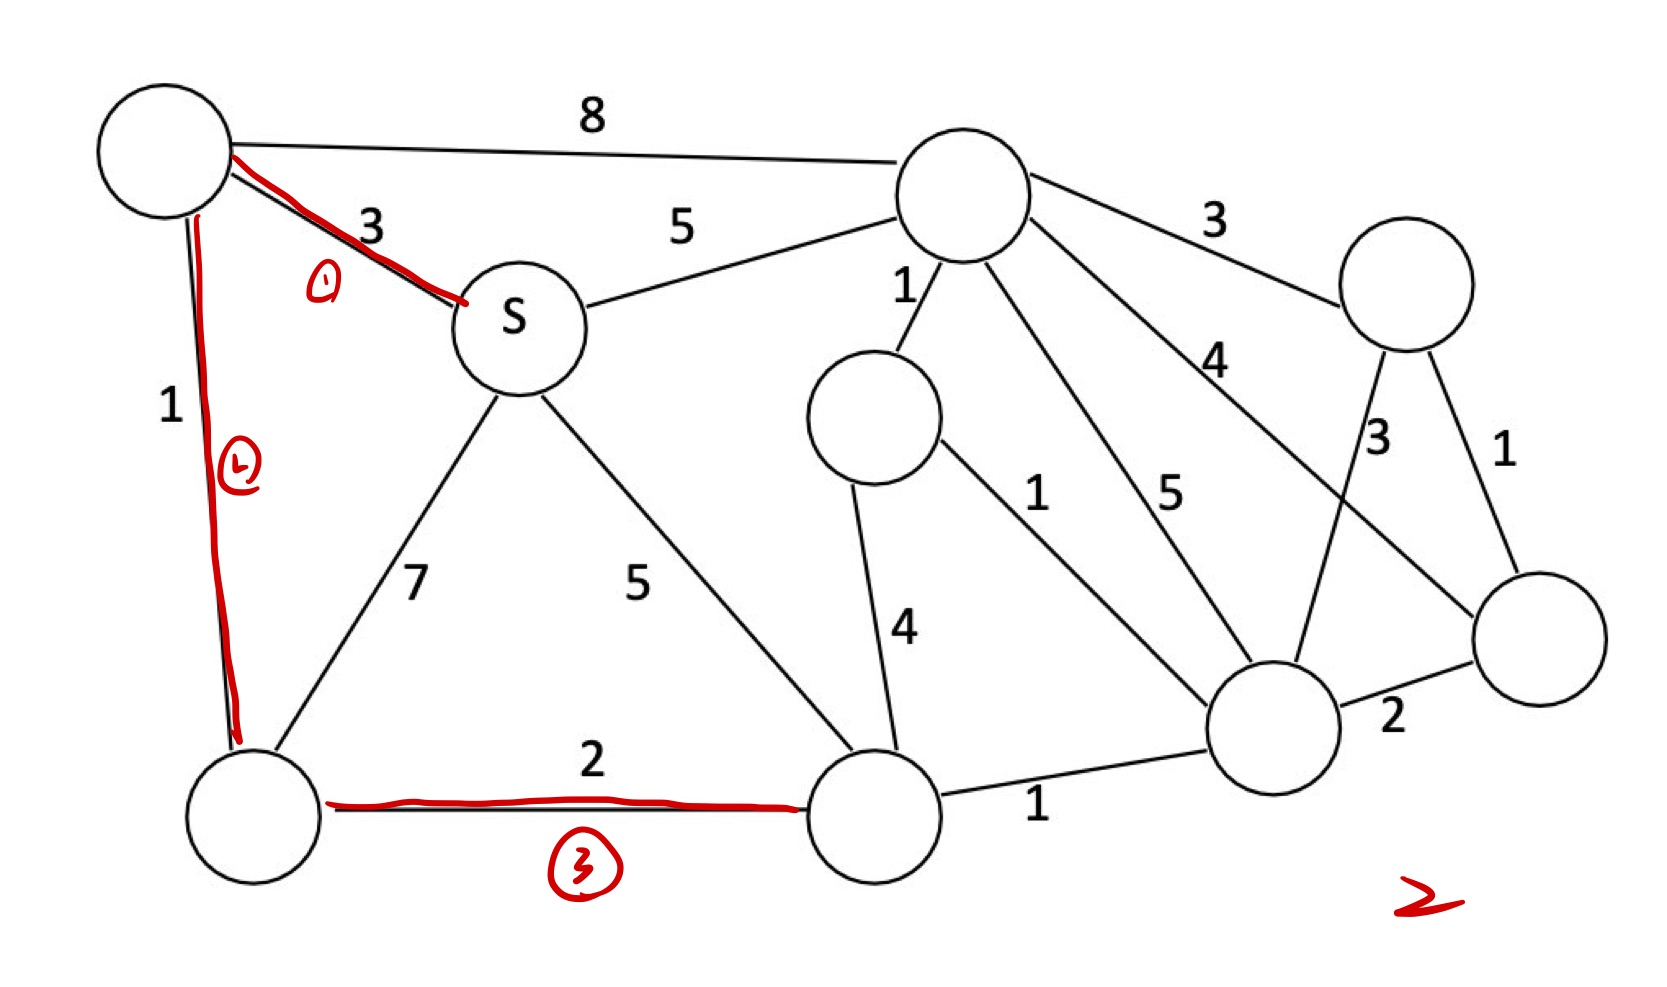
\includegraphics[width = 0.9\textwidth]{p7.jpg}
    \end{center}
        \end{sol}
        
        \item What is the value of the third edge chosen when finding a minimum spanning tree using Kruskal's algorithm?
        \begin{sol}
                \begin{center}
            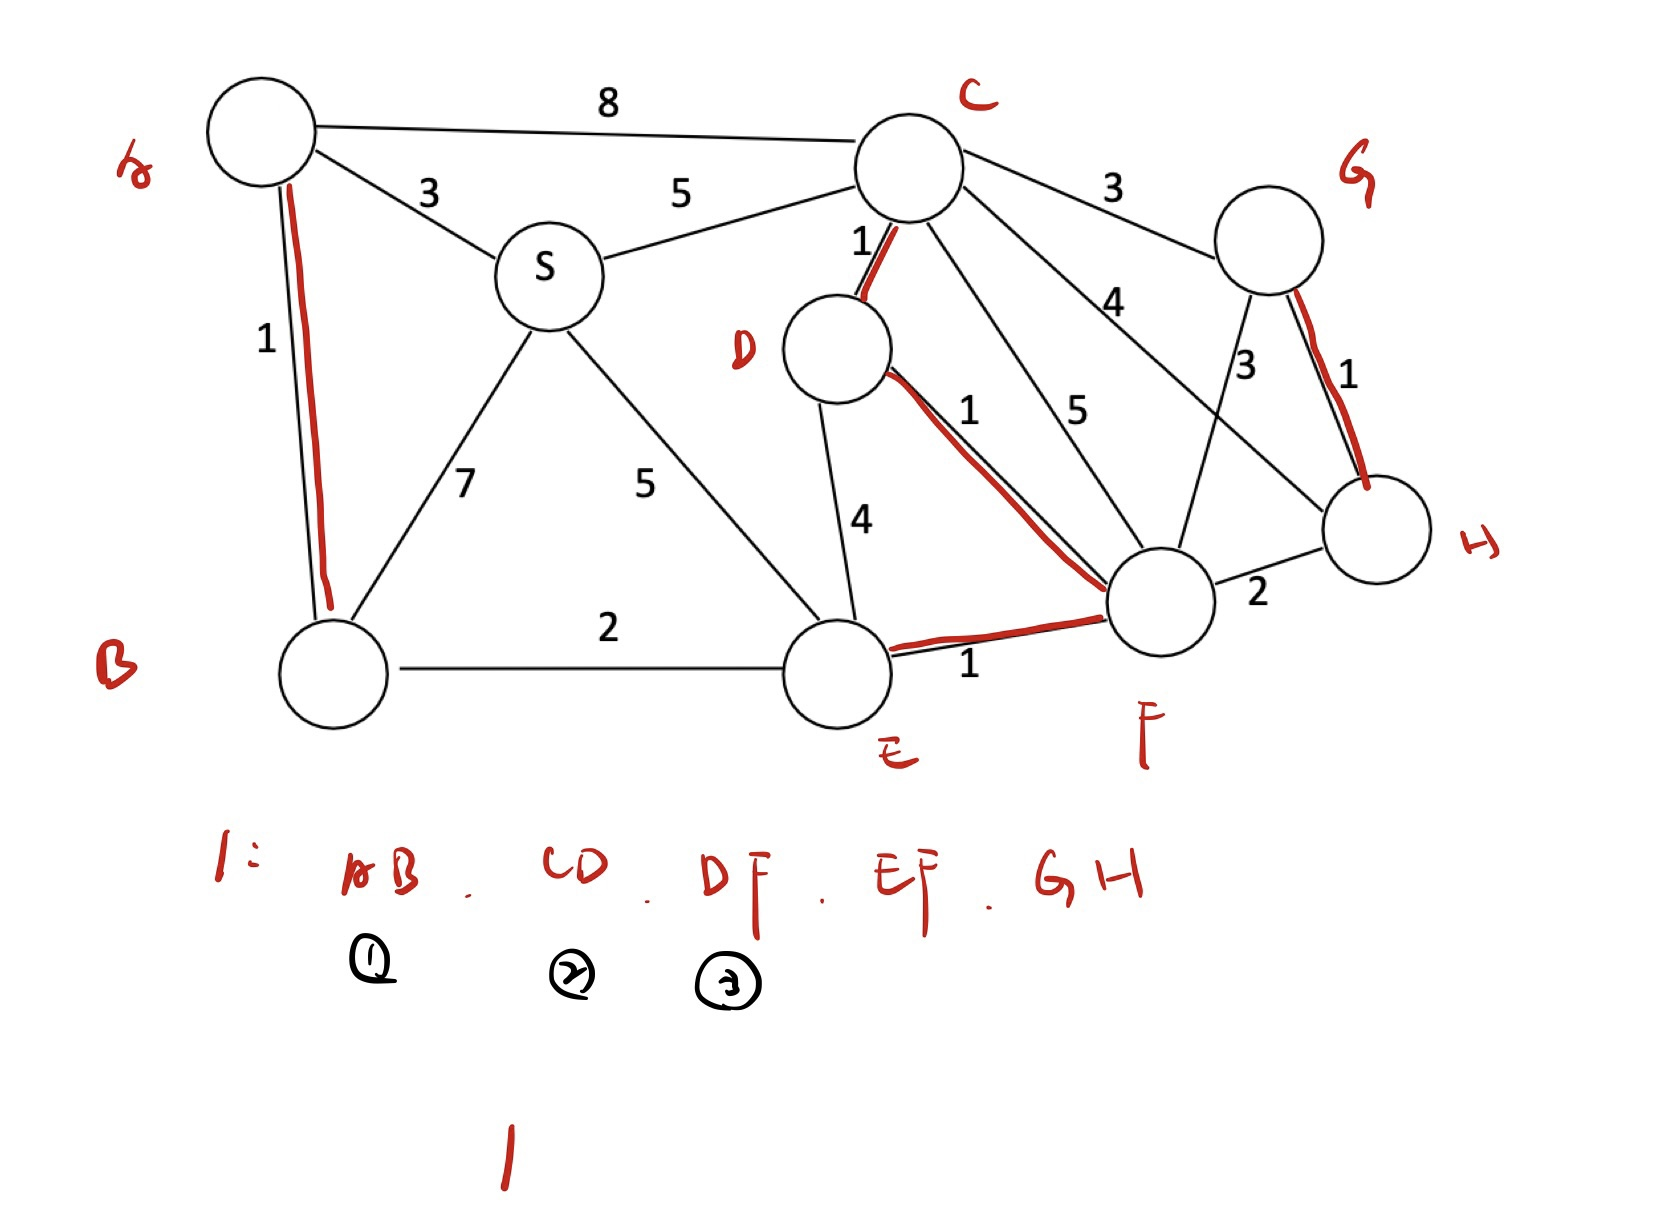
\includegraphics[width = 0.9\textwidth]{p8.jpg}
    \end{center}
        \end{sol}
        \item When using Dijkstra's algorithm to find the shortest path from S to all vertices, what is the value of the third edge chosen?
                \begin{sol}
                \begin{center}
            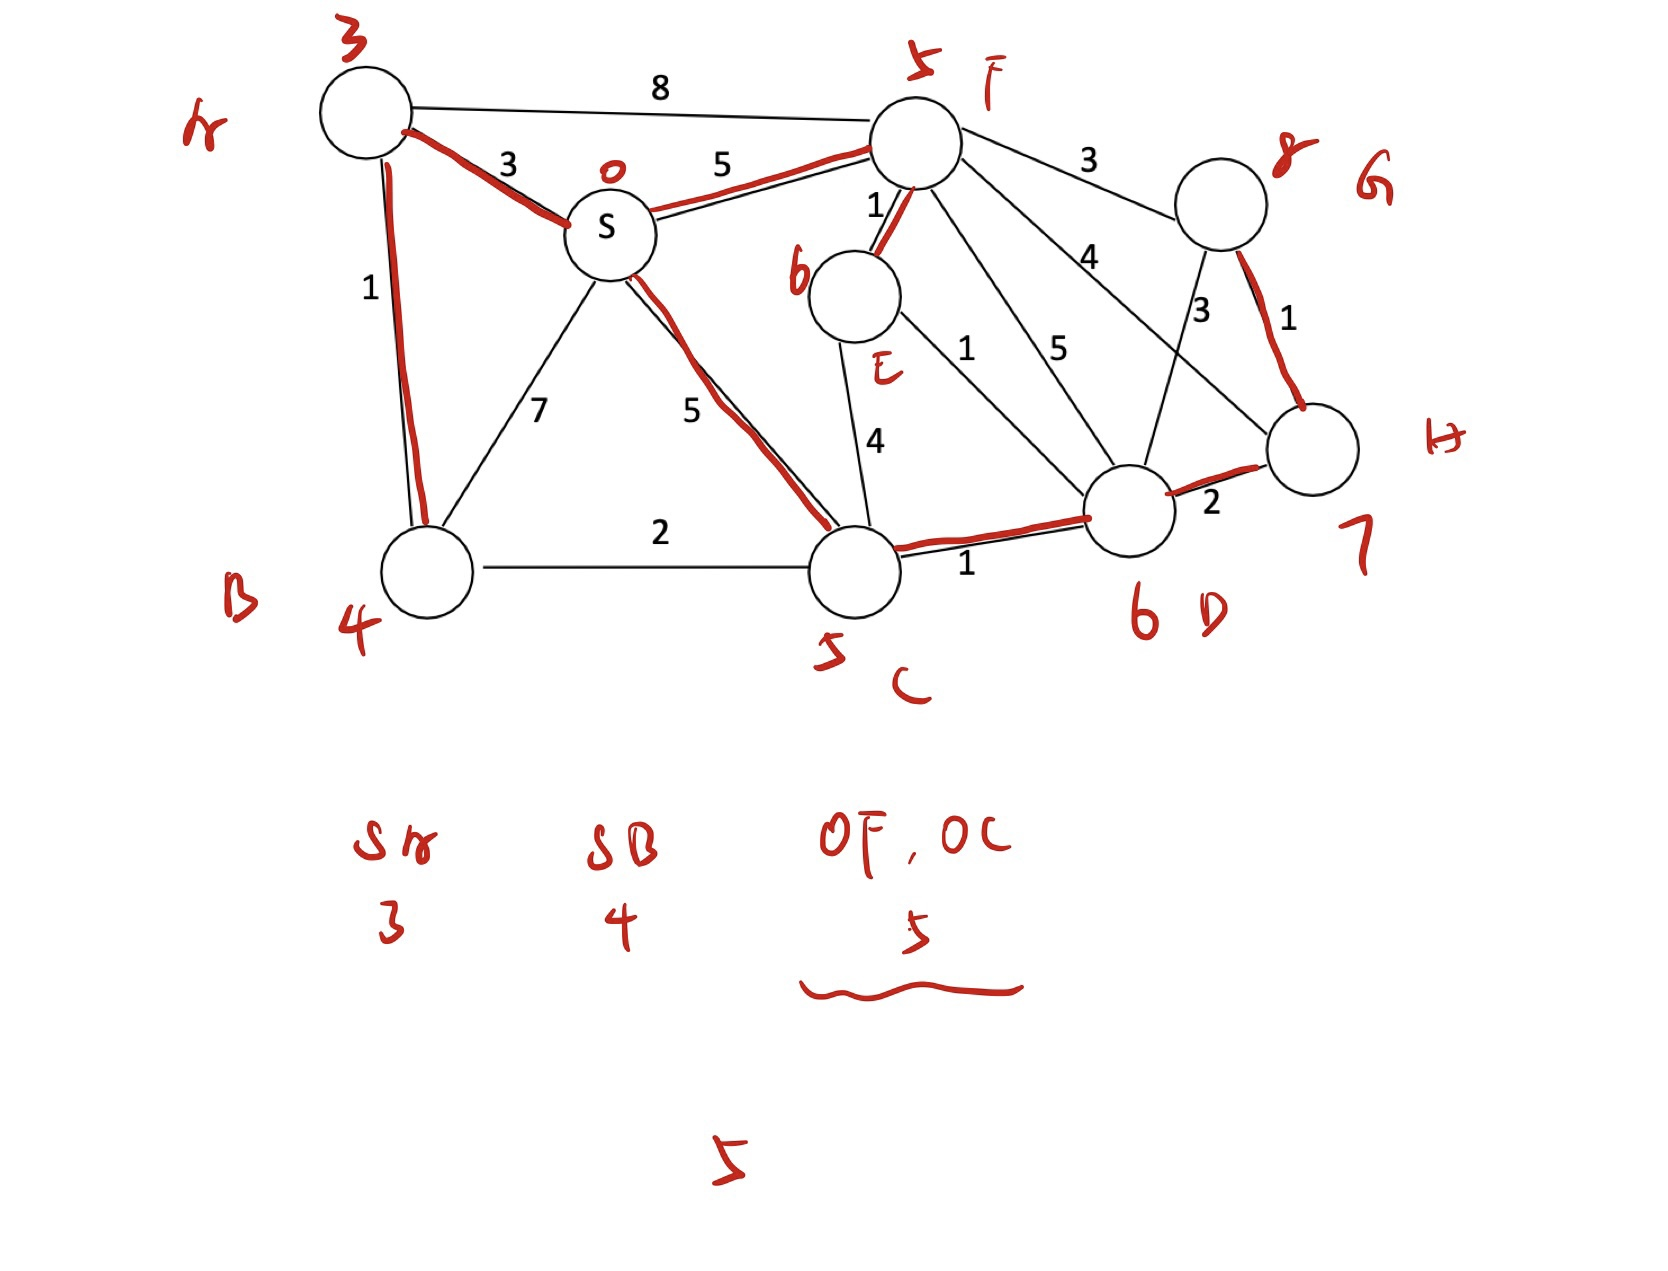
\includegraphics[width = 0.9\textwidth]{p9.jpg}
    \end{center}
        \end{sol}
        
        \item \textcolor{red}{How many components are in the graph?}
        \begin{sol}
            1 
        \end{sol}
        
        \item \textcolor{red}{What is the minimum number of edges you need to remove so the graph will have an Euler Tour? Mark the edges you would remove.}
        \begin{sol}
            Euler Tour: visit each edge exactly once and end up of your start vertex.\\
            3 \\
                            \begin{center}
            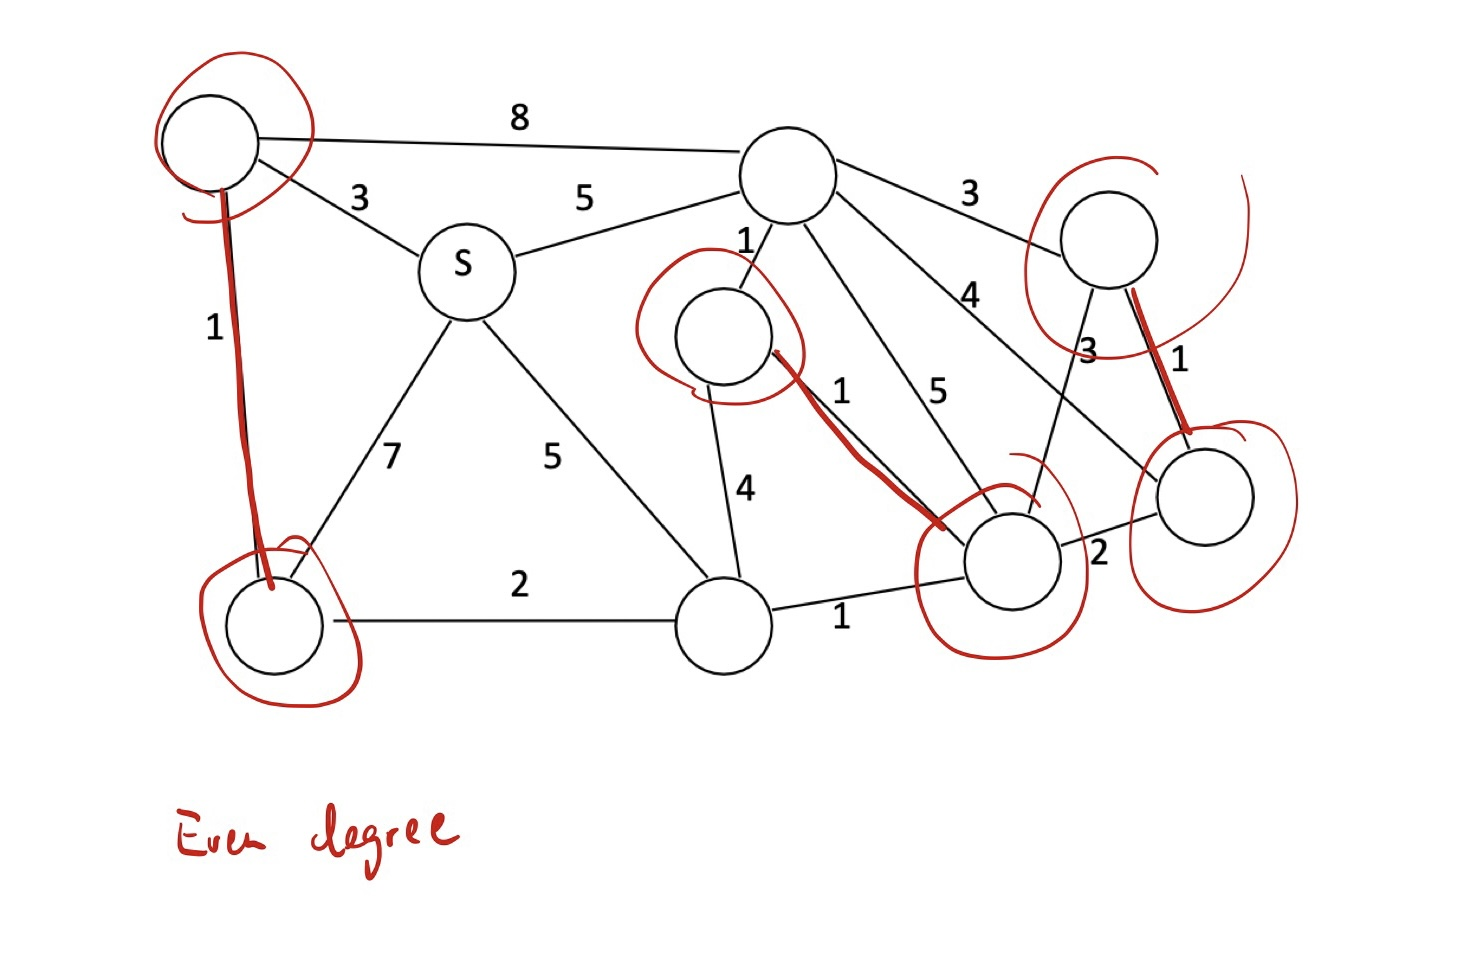
\includegraphics[width = 0.9\textwidth]{p10.jpg}
    \end{center}
        \end{sol}

    
    \end{enumerate}

    \item \ [6 pts] A particular problem requires 2 seconds to process 200 items and is $\Theta(n^3)$. You want to process 4000 items. You have a choice to either use a computer that is 10 times faster (allowing it to process 200 items in 0.2 seconds) or use the same computer with a different algorithm that still processes 200items in 2 seconds, but has a growth rate that is $\Theta(n^2)$.
    \begin{enumerate}
        \item Which is the faster choice for 4000 items?
        \begin{sol}
            Different 
        \end{sol}
        \item For what input sizes is the faster computer better?
        \begin{sol}
            $n < 2000$ \textcolor{red}{items}
        \end{sol}
        \item For what input sizes is the $\Theta(n^2)$ algorithm better?
        \begin{sol}
        $n>2000$ \textcolor{red}{items}
        \end{sol}
    \end{enumerate}

    \item \ \textcolor{red}{ [9 pts] You live in city G. You want to know the cost to travel from city G to all other cities (A,B,C,D,E,F‚H and I). The edges of the graph below represent the cost to travel the roads between various cities. If an edge doesn't exist, then there is no road between those two cities. In this particular scenario, even though the roads have a different cost, it takes most of a day to travel each road. Therefore, you must spend the night at each intermediate city (vertexa t an additional cost of 3.)}
    \begin{center}
            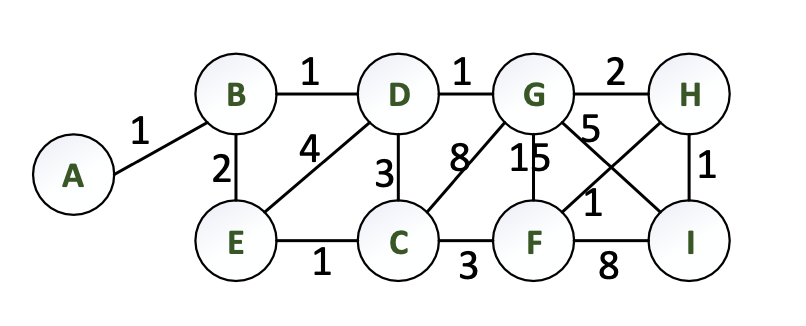
\includegraphics[width = 0.9\textwidth]{p11.png}
    \end{center}
    \begin{enumerate}

    \item How would you modify Dijkstra’s Single Source Shortest Path algorithm to find the cost from city G to all other cities in the graph with a vertex costing 3 to pass through it?
    \begin{sol}
        When passing through the city, the cost is 3 plus cost to reach the city instead of just the cost to reach the city.
    \end{sol}

    \item What is the order you reach the cities in your adjusted algorithm.
    \item Write the cost to reach each city from City G by its vertex in the graph.
    \begin{sol}
    (b) (c) \\ 
            \begin{center}
            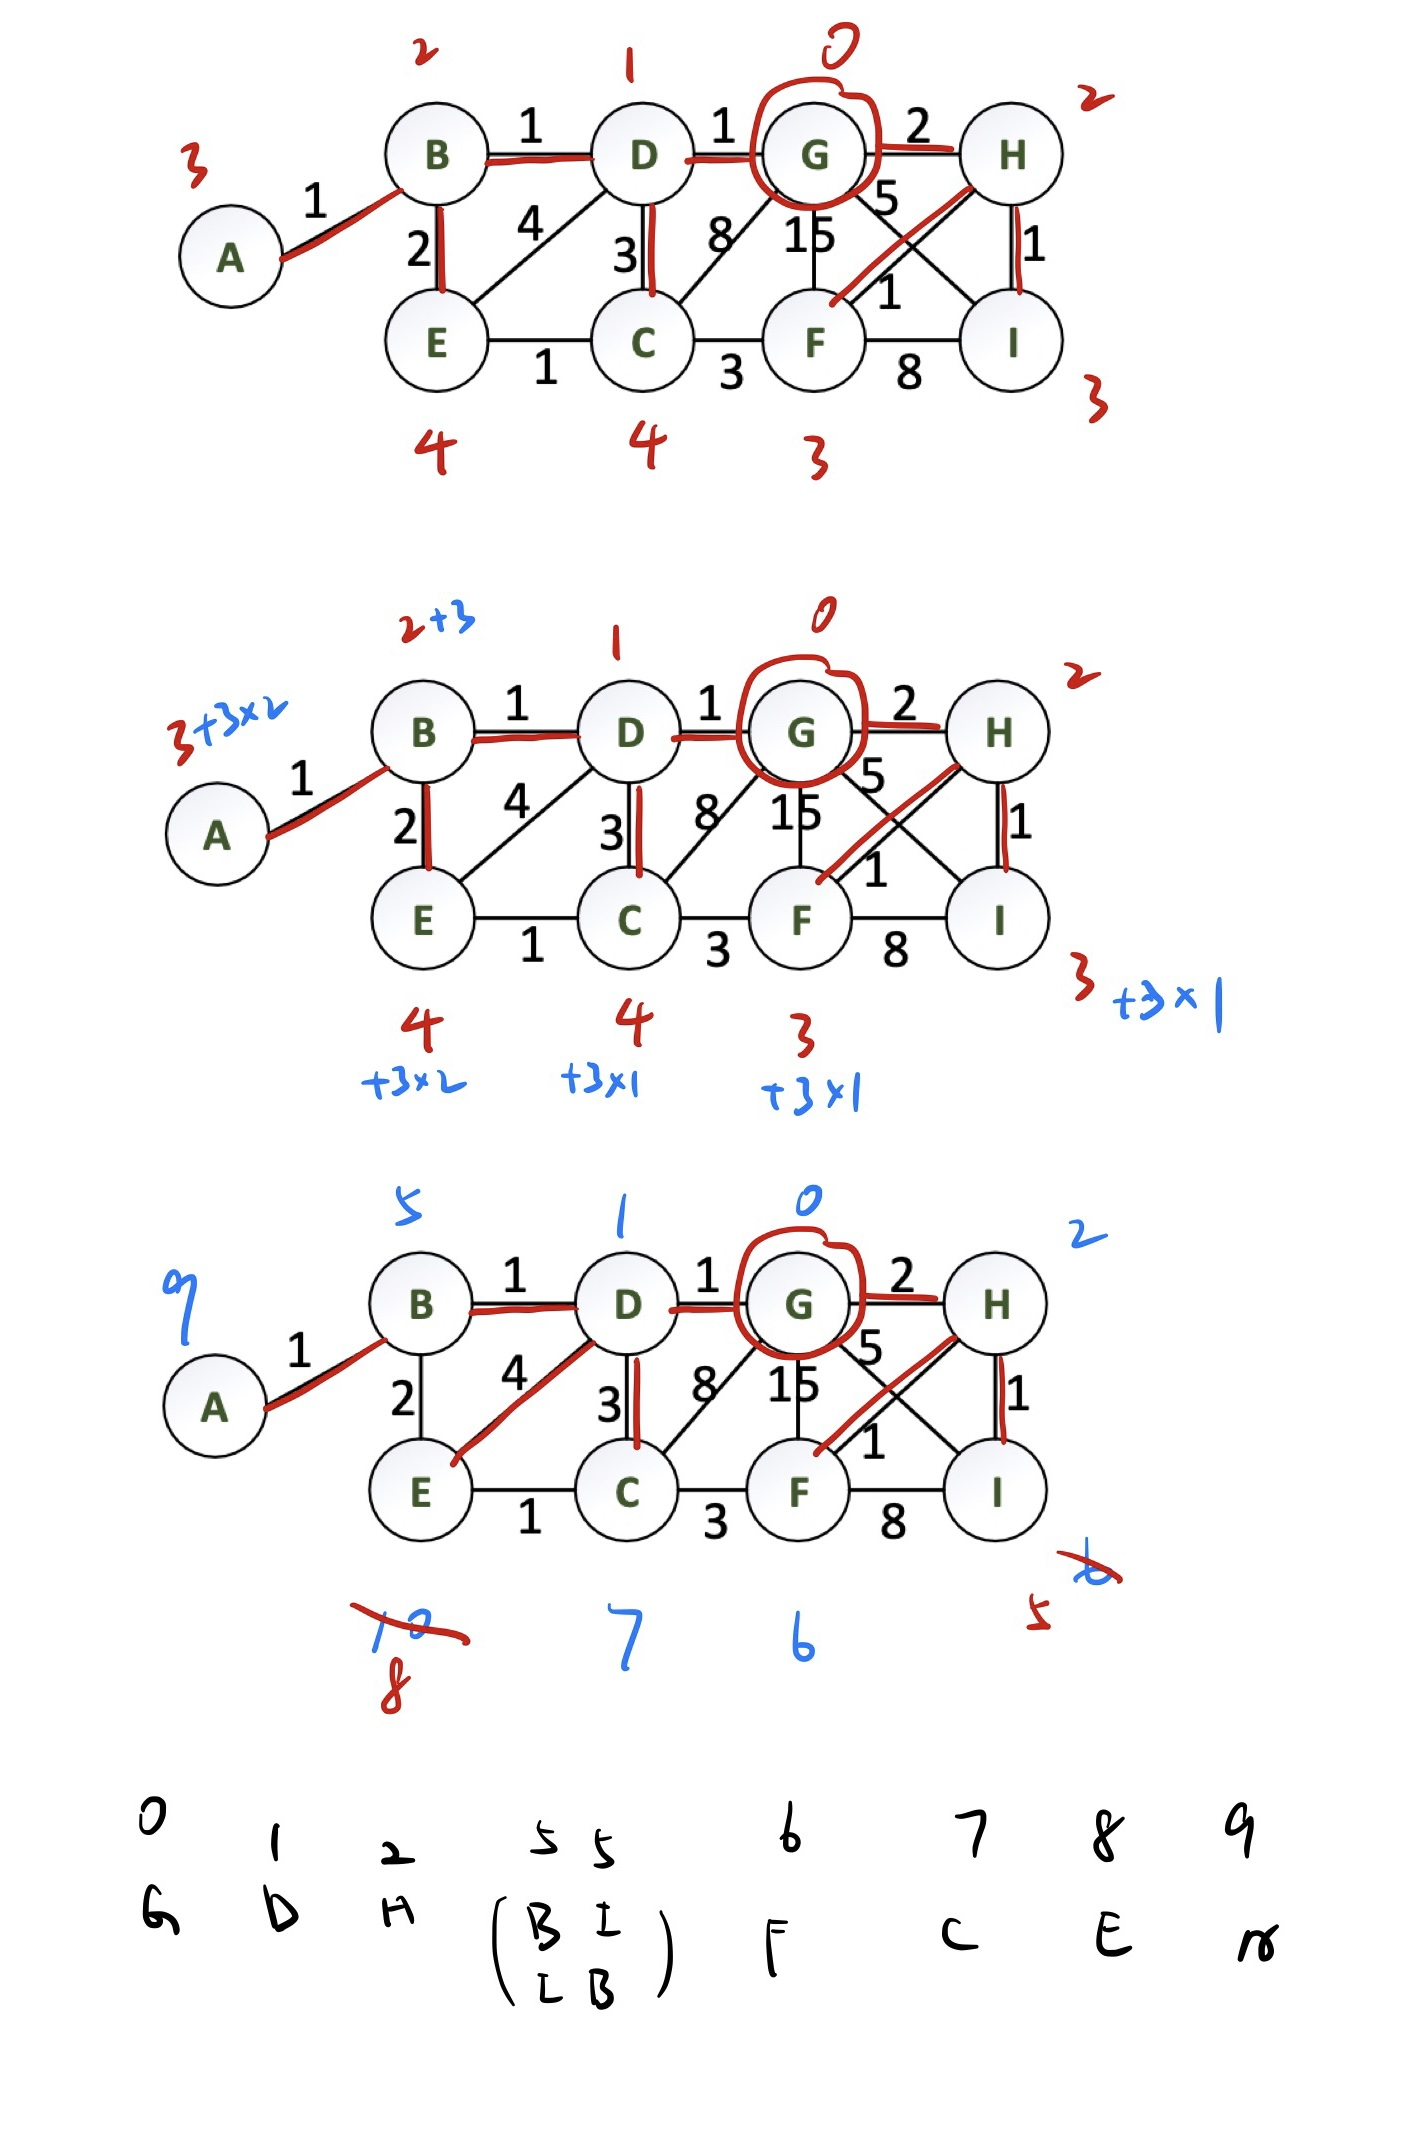
\includegraphics[width = 0.9\textwidth]{p12.jpg}
    \end{center}
    \end{sol}
    \end{enumerate}

    
\end{enumerate}

\end{document}
